% !TeX spellcheck = it_IT
\newpage
\section{Data Definition Language}
\subsection{Viste}
Le \textbf{Viste Logiche} possono essere definite come delle tabelle \textbf{virtuali}, i cui dati sono riaggregazioni dei dati contenuti nelle tabelle fisiche, senza contenerli effettivamente.\\
Le viste permettono di \textbf{semplificare} la rappresentazione dei dati ed evitare di ripetere query molto complesse. Forniscono inoltre un'ulteriore \textbf{sicurezza} in quanto si può fornire l'accesso di un utente solo ad esse e non a tutta la BD.\\
Hanno però alcune limitazioni:
\begin{itemize}
	\item Non è consentito usare \textbf{ORDER BY}
	\item A seconda del DBMS:
	\begin{itemize}
		\item Non si possono usare \textbf{UNION}, \textbf{INTERSECT} e \textbf{EXCEPT}
		\item \textbf{INTERSECT} e \textbf{EXCEPT} si possono realizzare con la \textbf{SELECT}
	\end{itemize}
\end{itemize}

\subsubsection{Creazione}
Si creano tramite il seguente comando:
\begin{lstlisting}[language=SQL]
	CREATE VIEW NomeVista [ ( ListaAttributi ) ] AS SelectSQL [ with [ local | cascaded ] check option ]
\end{lstlisting}
Si può scegliere di specificare i nuovi nomi delle colonne in \textbf{ListaAttributi}, altrimenti assumeranno gli stessi della tabella.

\begin{observation}[Viste di gruppo]
	Una vista di gruppo è una vista in cui una delle colonne è una funzione di gruppo. In questo caso è obbligatorio assegnare un nome alla colonna della vista corrispondente alla funzione.
\end{observation}

\subsubsection{Modifica}
Mentre il \textbf{contenuto} della vista è \underline{dinamico}, la sua \textbf{struttura} è \underline{statica}, quindi se viene aggiunta una colonna, questa non viene estesa alla vista.\\
Perché una vista sia \textbf{aggiornabile} (non strutturalmente ma a livello di contenuto), deve esistere una corrispondenza \textbf{biunivoca} tra le sue righe e quelle della tabella, ovvero:
\begin{itemize}
	\item \textbf{SELECT} senza \textbf{DISTINCT} e solo di attributi
	\item \textbf{FROM} una sola tabella modificabile
	\item \textbf{WHERE} senza SottoSelect
	\item Assenza di \textbf{GROUP BY} e \textbf{HAVING}
\end{itemize}
L'aggiornamento può essere utile nel caso in cui si vuole che degli utenti senza tutti i privilegi possano comunque fare modifiche limitate (e.g. l'amministrazione che può modificare il numero di telefono di un cliente). Per aggiornare si usa:
\begin{lstlisting}[language=SQL]
	INSERT INTO NomeVista (ListaAttributi) VALUES (ListaValori)
\end{lstlisting}
\paragraph{Controllo dell'aggiornamento}
Se si prevede che la view sia modificabile, alla sua creazione va aggiunto \textbf{WITH CHECK OPTION}. Questo garantisce che eventuali inserimenti saranno permessi solo se soddisfano la clausola \textbf{WHERE} specificata alla creazione. \textbf{LOCAL} e \textbf{CASCADE} consentono di decidere nel caso in cui la vista sia creata sulla base di un'altra, se è necessario controllare o meno tutte le clausole \textbf{WHERE}.

\subsubsection{Eliminazione}
Viene utilizzato il seguente comando
\begin{lstlisting}[language=SQL]
	DROP VIEW nome_view {RESTRICT/CASCADE}
\end{lstlisting}
Dove \textbf{RESTRICT} indica che la view viene eliminata solo se non è riferita da altri oggetti mentre \textbf{CASCADE} elimina anche tutte le altre dipendenze da essa.

\subsection{Trigger}
Un trigger definisce un’azione che il database deve attivare automaticamente quando si verifica un determinato \textbf{evento} nella BD, ovvero determinati comandi quali:
\begin{itemize}
	\item Comandi \textbf{DML} quali INSERT, UPDATE e DELETE
	\item Negli ultimi DBMS anche comandi \textbf{DDL} come CREATE VIEW
	\item Aggiornamenti di specifiche colonne
\end{itemize}
Un trigger può essere:
\begin{itemize}
	\item \textbf{Attivo} se modifica lo stato della BD
	\item \textbf{Passivo} se provoca solo il fallimento della transazione in certi casi
\end{itemize}

\subsubsection{Granularità}
I trigger possono essere eseguiti su due livelli:
\begin{itemize}
	\item \textbf{Riga}: vengono eseguiti una volta per ogni riga modificata nella transazione. Spesso utilizzati per \textbf{audit} dei dati e per \textbf{sincronizzazione}. Va specificato con
	\begin{lstlisting}[language=SQL]
		FOR EACH ROW
	\end{lstlisting}
	\item \textbf{Istruzione}: vengono eseguiti una volta per transazione. Sono usati Per attività correlate ai dati (e.g. sicurezza)
\end{itemize}

\subsubsection{Creazione}
La struttura di un comando di creazione di un trigger è la seguente:
\begin{lstlisting}[language=SQL]
	CREATE TRIGGER Nome
	BEFORE/AFTER INSERT/DELETE/UPDATE of ATTRIBUTI {, Evento}
	ON Tabella [WHEN Condizione]
	FOR EACH {ROW/STATEMENT}
	Azione
\end{lstlisting}

\subsubsection{INSTEAD OF}
Questo comando può essere usato per eseguire un'azione diversa invece di quella che dovrebbe succedere con l'evento previsto. Può essere usato anche sulle viste ma deve per forza essere a livello di riga.

\newpage
\subsection{Accessi}
Ogni \textbf{risorsa} dello schema può essere protetta dal creatore della risorsa. Il creatore della DB, salvo sue diverse specifiche, è l'unico a poter eseguire \textbf{CREATE}, \textbf{ALTER} e \textbf{DROP} ed è l'unico a poter garantire o rimuovere privilegi.

\subsubsection{Concessione}
\begin{lstlisting}[language=SQL]
	GRANT Privilegi ON Oggetto TO Utenti [ WITH GRANT OPTION ]
\end{lstlisting}
\textbf{WITH GRANT OPTION} specifica se il privilegio può essere trasmesso o meno ad altri utenti.

\subsubsection{Revoca}
\begin{lstlisting}[language=SQL]
	REVOKE [ GRANT OPTION FOR ] Privileges ON Resource FROM Users [ RESTRICT | CASCADE ]
\end{lstlisting}
Il comando revoca quei privilegi anche a chiunque li abbia ricevuti da quell'utente. \textbf{RESTRICT} indica che il comando non deve essere eseguito se comporterebbe la revoca di qualcos'altro mentre \textbf{CASCADE} ne forza l'esecuzione.

\subsubsection{Grafo autorizzazioni}
È il grafo che rappresenta quali autorizzazioni sono state concesse e da chi. Se un nodo $N$ ha un arco uscente con un privilegio, allora esiste un cammino da SYSTEM a $N$ con ogni arco etichettato dallo stesso privilegio WITH GRANT OPTION.

\begin{example}
	Ogni utente ($A$, $B$, $C$, $I$) esegue una serie di comandi:
	\begin{lstlisting}[language=SQL]
		I: GRANT SELECT ON R TO A WITH GRANT OPTION
		A: GRANT SELECT ON R TO B WITH GRANT OPTION
		B: GRANT SELECT ON R TO A WITH GRANT OPTION
		I: GRANT SELECT ON R TO C WITH GRANT OPTION
		C: GRANT SELECT ON R TO B WITH GRANT OPTION
		
		I: REVOKE SELECT ON R FROM A CASCADE
		
		I: REVOKE SELECT ON R FROM C CASCADE
	\end{lstlisting}
	\begin{figure}[!h]
		\centering
		\begin{minipage}{.3\textwidth}
			\centering
			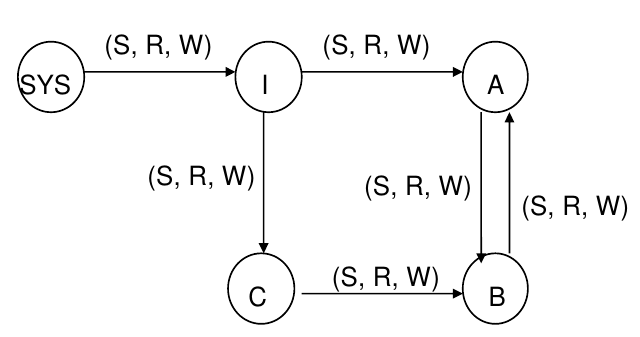
\includegraphics[scale=0.2]{grafo1.png}
			\captionof{figure}{GRANT}
		\end{minipage}
		\begin{minipage}{.3\textwidth}
			\centering
			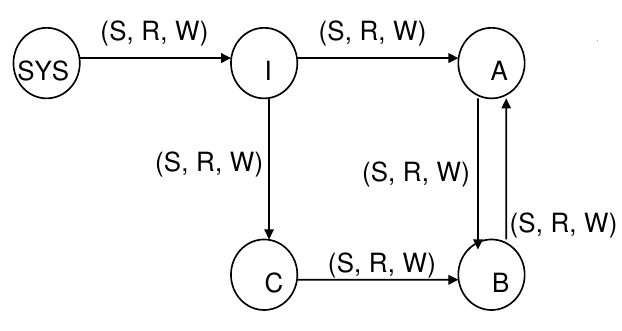
\includegraphics[scale=0.2]{grafo2.png}
			\captionof{figure}{Prima REVOKE}
		\end{minipage}
		\begin{minipage}{.3\textwidth}
			\centering
			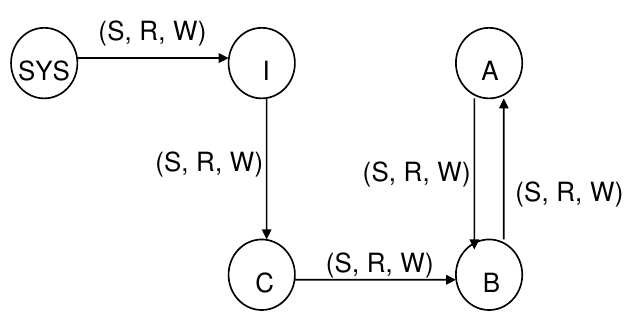
\includegraphics[scale=0.2]{grafo3.png}
			\captionof{figure}{Seconda REVOKE}
		\end{minipage}
	\end{figure}
\end{example}

\subsection{Indici}
Gli Indici sono strutture dati che vengono create su tabelle per eseguire alcune query più velocemente. Non essendo un comando standard può avere varie sintassi:
\begin{lstlisting}[language=SQL]
	CREATE INDEX NomeIdx ON Tabella(Attributi)
	CREATE INDEX NomeIdx ON Tabella	WITH STRUCTURE = BTREE, KEY = (Attributi)
	DROP INDEX NomeIdx
\end{lstlisting}

\newpage
\subsection{Catalogo dei metadati}
Il catalogo dei metadati consiste in un insieme di tabelle di sistema. Alcuni esempi sono:
\begin{itemize}
	\item Delle \textbf{password}
	\begin{lstlisting}[language=SQL]
		PASSWORD(username, password)
	\end{lstlisting}
	\item Delle \textbf{BD}
	\begin{lstlisting}[language=SQL]
		SYSDB(dbname, creator, dbpath, remarks)
	\end{lstlisting}
	\item Delle \textbf{tabelle} e \textbf{view} (type)
	\begin{lstlisting}[language=SQL]
		SYSTABLES(name, creator, type, colcount, filename, remarks)
	\end{lstlisting}
	\item Degli \textbf{attributi}
	\begin{lstlisting}[language=SQL]
		SYSCOLUMNS(name, tbname, tbcreator, colno, coltype, lenght, default, remarks)
	\end{lstlisting}
	\item Degli \textbf{indici}
	\begin{lstlisting}[language=SQL]
		SYSINDEXES(name, tbname, creator, uniquerule, colcount)
	\end{lstlisting}
\end{itemize}